\documentclass{article}
\usepackage[T2A]{fontenc}
\usepackage[utf8]{inputenc}
\usepackage[russian]{babel}
\usepackage{amsmath}
\usepackage{amsmath}
\usepackage{wrapfig}
\usepackage{graphicx}

\begin{document}

\begin{wrapfigure}{l}{0.3\textwidth}
  \centering
  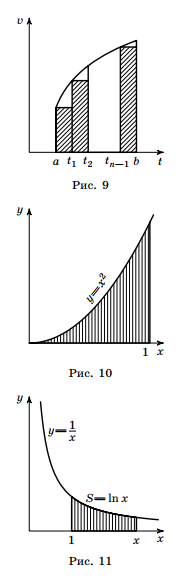
\includegraphics[width=0.25\textwidth]{4_pictures.png}
\end{wrapfigure}

Примем для удобства \( t_0 = a \), \( t_n = b \).

\begin{center}
    \textbf{Рис. 9}
\end{center}

Площадь \( S \), о которой идёт речь, с любой точностью можно заменить на сумму площадей прямоугольников с нижними основаниями \([t_0, t_1]\), \([t_1, t_2]\), ..., \([t_{n-1}, t_n]\) и с высотами \( v(t_0) \), \( v(t_1) \), ..., \( v(t_{n-1}) \), т.е. получаем
\[
S \approx v(t_0)(t_1 - t_0) + v(t_1)(t_2 - t_1) + \dots + v(t_{n-1})(t_n - t_{n-1}) = \sum_{k=0}^{n-1} v(t_k)(t_{k+1} - t_k) = \sum_{k=0}^{n-1} v(t_k) \Delta t_k
\]
(это сокращённое обозначение левой части).

Более точная запись:
\[
S = \lim_{\Delta t_k \to 0, \, n \to \infty} \sum_{k=0}^{n-1} v(t_k)(t_{k+1} - t_k) = \lim_{\Delta t_k \to 0, \, n \to \infty} \sum_{k=0}^{n-1} v(t_k) \Delta t_k,
\]
где \( \Delta t_k = t_{k+1} - t_k \). Можно, например, брать разбиение отрезка \([a, b]\) на \( n \) равных частей, так что \( \Delta t_k = \frac{b-a}{n} \), и тогда условие перехода к пределу состоит просто в том, что \( n \to \infty \).

Но, с другой стороны, точно так же можно находить путь, пройденный в промежутке от \( a \) до \( b \), так как на маленьких участках \([t_k, t_{k+1}]\) скорость можно считать постоянной. Итак,
\[
S = \int_{a}^{b} v(t) \, dt = \lim_{\Delta t_k \to 0, \, n \to \infty} \sum_{k=0}^{n-1} v(t_k) \Delta t_k.
\]

Отметим соглашение о знаке площади: если кусок площади лежит под осью абсцисс, то его знак считается отрицательным, так как в этом случае \( \Delta t_k > 0 \), а \( v(t_k) < 0 \).

\textbf{Пример 1.} Найдём площадь \( S \) под параболой \( y = x^2 \) от точки \( x = 0 \) до точки \( x = 1 \) (рис. 10). Имеем:
\[
S = \int_{0}^{1} x^2 \, dx = \left. \frac{x^3}{3} \right|_{0}^{1} = \frac{1}{3}.
\]

\textbf{Пример 2.} Площадь под гиперболой \( y = \frac{1}{x} \) от \( x = 1 \) до произвольного \( x \) равна
\[
\int_{1}^{x} \frac{1}{t} \, dt = \ln t \Big|_{1}^{x} = \ln x.
\]

Таков геометрический смысл натурального логарифма.

\end{document}
